\epigraph{The difference between ideas and reality is the
difference between philosophy and engineering. The work to transform one into
the other is scientific research}{{\itshape V-Research}}
\begin{figure}[t]
	\centering
	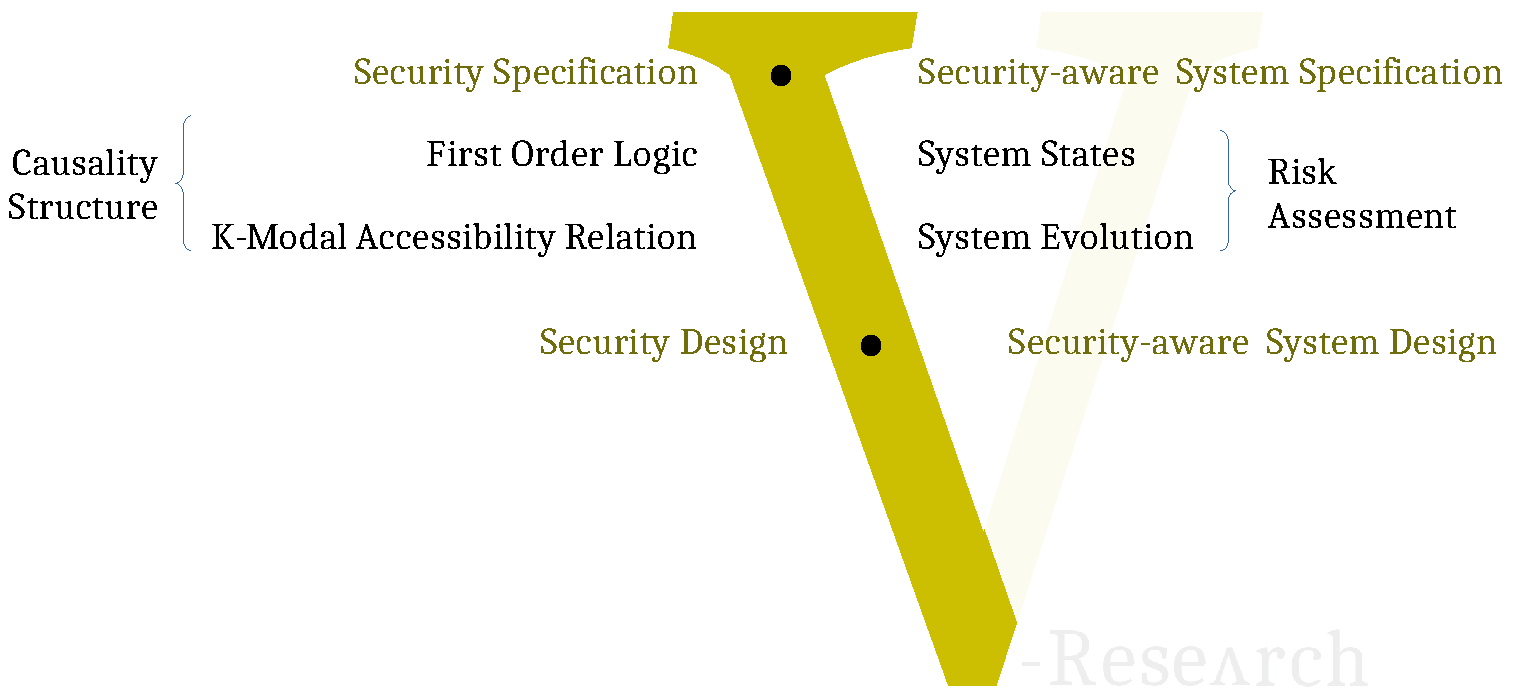
\includegraphics[width=\textwidth]{vmodel.pdf}
	\caption{Cybersecurity Engineering Life-cycle}
	\label{fig:knowledge-belief}
\end{figure}

\subsection{Elicitation of Security Requirements}\label{sec:properties}
Infosec, or Information Security, aims at mitigating the security
risks related to information. The standard de-facto is 
the so called CIA triad (where CIA stands for Confidentiality, Integrity, Availability).

Confidentiality: the information is accessible only to authorised individuals.
A set of rules that limits access to information.  The information can be
accessed by X if and only if X is authorized to access it = X has the right
attributes (i.e. keys, password) to access it.

Integrity: the information is trustworthy and accurate (i.e. uncorrupted and
unaltered). Protects data from modification or deletion by unauthorized sources
and the ability to undo any damage done.  (for data at rest) If the information
X is written, A will always be read. If information X is modified to
information X', information X can always be recovered.  (for data in transit)
If the information X is sent, A will be received. If information X is modified
to information X', information X can always be recovered.

Availability: the information is accessible and usable when required. Guarantee
of reliable access to the information by authorized people If the information X
needs to be accessed, information X can be retrieved. If

Authenticity: assurance that the information is from the source it claims to be
from. Authenticity involves proof of identity. Authenticity is verified through
authentication.  If information X arrives from A to B, A sent information X and
B can verify it.  ??Authenticity implies integrity but Integrity doesn't imply
authenticity??  ??Authenticity doesn't imply confidentiality but
confidentiality does imply authenticity??

Non-repudiation: the ability to ensure that a party to a contract or a
communication cannot deny the authenticity of their signature on information
(or the sending of) that they originated.  If information X arrives from A, A
sent it and cannot deny it (partial overlap??).  If sender A sends information
X, it cannot say he didn't do it.  Non-repudiation implies authenticity and
integrity. Authenticity doesn't imply non-repudiation (replay attacks?).
Integrity doesn't imply non-repudiation (replay attacks?). 

\subsubsection{Relevant Standards}\label{sec:standards}
\begin{enumerate}[noitemsep]
	\item DO-326A
\end{enumerate}

\begin{enumerate}
\item specification -- definition of the desired design of a system. The
specification is verified w.r.t. the  $\abf$ theory. Checking the
controls of the whole cybersecurity life-cycle and the relation with
CWE.
\item design -- the mitigations identified in the specification stage
are implemented into the design. The security of the assets w.r.t. the design are
verified with a, so called, cybersecurity risk assessment.
\end{enumerate}
